%\UseRawInputEncoding
\documentclass{article}
\setcounter{secnumdepth}{0}
\usepackage[T1]{fontenc}
\usepackage[utf8]{inputenc}
%\usepackage[latin1]{inputenc}
%\usepackage[english, norsk]{babel}
\usepackage{filecontents}
\usepackage{tcolorbox}
\usepackage{url}
\usepackage{etoolbox}
\usepackage{framed}
\usepackage{framed, color}
\usepackage{xcolor}
\usepackage{mdframed}
\usepackage{float}
\usepackage{gensymb}
\usepackage{amsmath}

\definecolor{Black}{rgb}{0.0, 0.0, 0.0}

%Definer kode
\usepackage{listings}
\usepackage{color}
\definecolor{dkgreen}{rgb}{0,0.6,0}
\definecolor{gray}{rgb}{0.5,0.5,0.5}
\definecolor{mauve}{rgb}{0.58,0,0.82}

\lstset{frame=tb,
extendedchars = true,
texcl=true,
  language=C++,
  aboveskip=3mm,
  belowskip=3mm,
  showstringspaces=false,
  columns=flexible,
  basicstyle={\small\ttfamily},
  numbers=none,
  numberstyle=\tiny\color{gray},
  keywordstyle=\color{blue},
  commentstyle=\color{dkgreen},
  stringstyle=\color{mauve},
  breaklines=true,
  breakatwhitespace=true,
  tabsize=3
}

\usepackage[colorlinks]{hyperref}
\hypersetup{citecolor=Black}
\hypersetup{linkcolor=Black}
\hypersetup{urlcolor=Black}
\usepackage{cleveref}


\setlength{\parindent}{0em}
\setlength{\parskip}{1em}
%\renewcommand{\baselinestretch}{2.0}

%\renewcommand\thesubsection{\alph{subsection}}

\renewcommand{\figurename}{Figure}
\begin{document}
\author{Kent Odde}
\title{Title}

\maketitle
\thispagestyle{empty}
\begin{center}
\includegraphics[width=\linewidth,height=0.2\textheight,keepaspectratio]{img/USN.png}
\end{center}
\newpage

\tableofcontents

\newpage

\section{Abstract}
This is my submission for the home exam in Discrete Mathmatics, fall 2020. The assignment consists of implementing the ElGamal encryption algorithm, in a programming language of my own choosing. 


Quite a bit of overhead were required to encrypt larger inputs. Because this course is concerned with the mathematics behind ElGamal and to satisfy the professors requirement for a short paper, I will not cover this part of the implementation to a detailed extent. 

%Innholdsfortegnelse
\section{Introduction}


%Implementation
\section{Implementation}
\subsection{Finding and choosing a generator}

\begin{equation}
Y = g^{x} \bmod p
\end{equation}

	For every value of x, we should get a unique value of Y

	All generators are factors of p-1


\subsection{Overhead}

\subsection{Padding}
	PKCS\#1.5
	%https://www.di-mgt.com.au/rsa_alg.html

Asymmetric encryption algorithms like RSA and ElGamal, requires a padding scheme in order to increase the security. A common padding scheme for RSA is PKCS\#1.5. As it was hard to find sources for padding schemes commonly used with ElGamal, my choice also fell on PKCS for this implementation. 


A visualization of the scheme can be seen in figure XX.  


\begin{figure}[H]
 \centering
  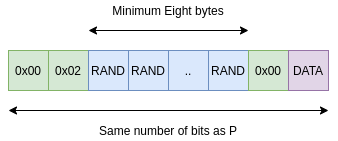
\includegraphics[width=300pt]{img/padding.png}
 \caption{PKCS padding scheme}
 \end{figure}

\subsection{Block Handling}

ElGamal is not a common choice for encrypting larger texts, however after conversations with the lecturer, I understood that this was a requirement for this assignment. To keep the overhead to a minimum ECB(Electronic Codebook) was chosen. An illustration of ECB can be seen in figure XX. If the plaintext is larger than the number of bits of P, we divide it up into blocks, encrypt them seperately, and concatenate them. 


\begin{figure}[H]
 \centering
  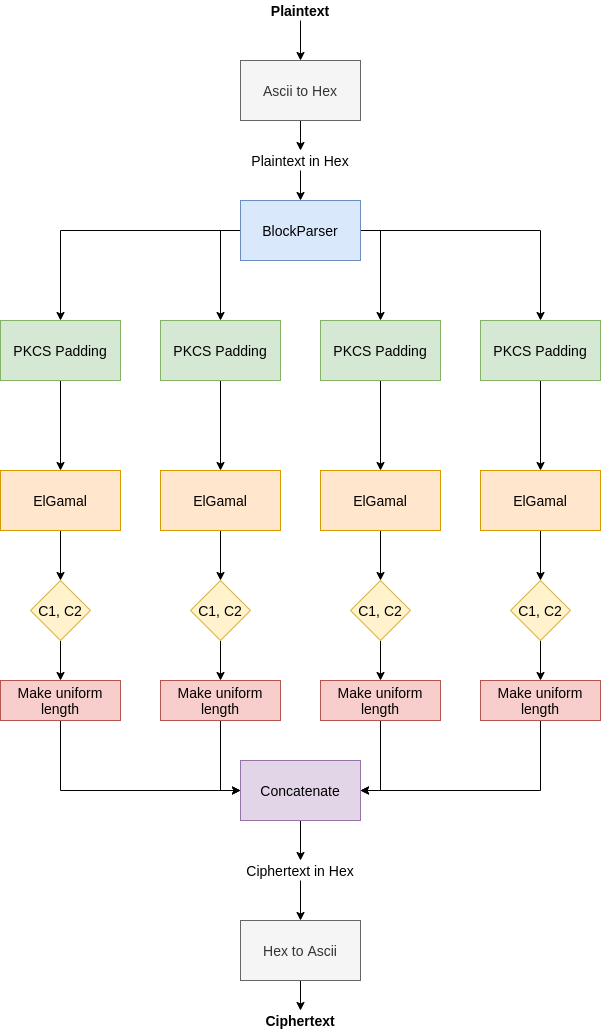
\includegraphics[width=300pt]{img/overview.png}
 \caption{PKCS padding scheme}
 \end{figure}

An extra complication with ElGamal is that the algorithm produces two numbers, in which the size of bits may vary. In order to be able to parse the concatenated strings later, I decided to prepend zeroes to c1 and c2, until their length were at 512 bits.
%Konklusjon
\section{Conclusion}

\begin{figure}[H]
 \centering
  
\includegraphics[width=300pt]{img/usn.png}
 \caption{..}
 \end{figure}




%Vedlegg
\section{Appendices}


\newpage
%Referanse
%\section{Referanser}

\nocite{*}
\bibliographystyle{plain}
\bibliography{ref}

\addcontentsline{toc}{section}{References}

\end{document}